\section{Theorie}
\label{sec:Theorie}

Ein Geiger-Müller-Zählrohr ist eine Apparatur, mit der die Intensität ionisierter Strahlung gemessen werden kann.
Ein schematischer Aufbau ist in \hyperref[fig:Aufbau1]{Abbildung \ref{fig:Aufbau1}} dargestellt.
\begin{figure} [H]
    \center
    \caption{Schematischer Aufbau eines Zählrohres}\label{fig:Aufbau1}
    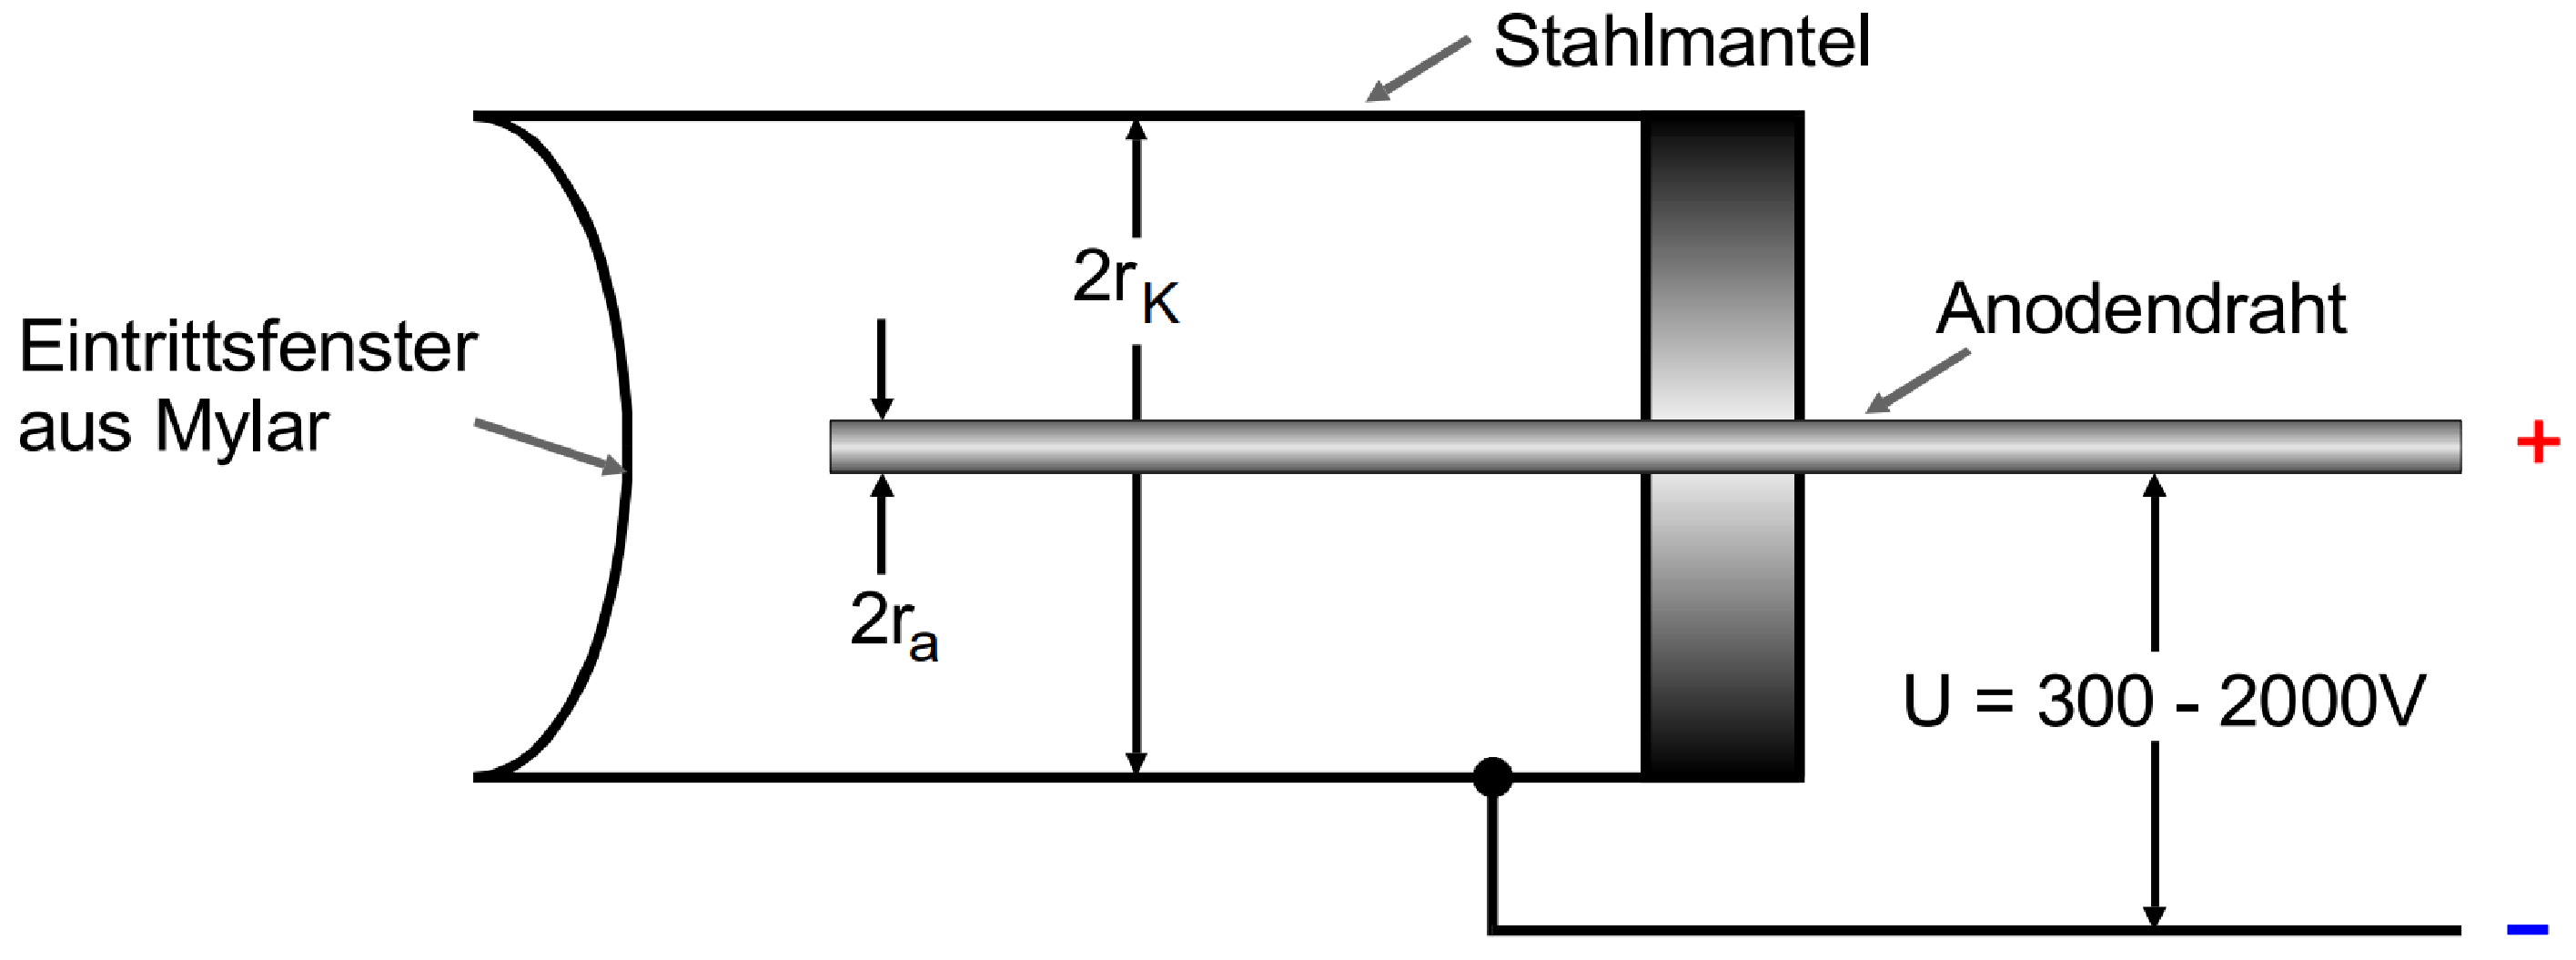
\includegraphics[width=0.7\linewidth]{pictures/Aufbau1.pdf}
\end{figure}
